\begin{frame}{Programy wywoławcze}

	Poniższe programy wywołuje się z linii poleceń z odpowiednimi argumentami.

	\begin{itemize}
		\myitem {\large \textbf{Play}}
		\begin{itemize}
			\item Rozpoczyna rozgrywkę między graczami (każdy z nich może być człowiekiem lub komputerem)
			\item Dla graczy komputerowych należy podać również pliki z ciągiem wag
			\item I/O na poziomie konsoli
		\end{itemize}
		\myitem {\large \textbf{Find}}
		\begin{itemize}
			\item Rozpoczyna sesję algorytmu genetycznego
			\item Może wznowić przedwcześnie przerwaną sesję z pliku populacji
			\item Wynik zapisuje w \textbf{heuristics/output/}
		\end{itemize}
		\myitem {\large \textbf{Show}}
		\begin{itemize}
			\item Nazwa pliku osobnika do wyświetlenia
		\end{itemize}
	\end{itemize}

    % \begin{columns}

	% 	\begin{column}{.4\hsize}
	% 		\begin{figure}
	% 			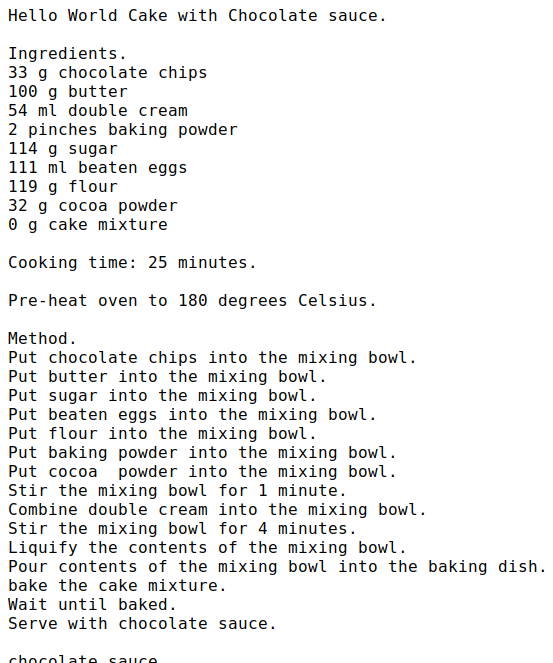
\includegraphics[height=6cm]{figures/chef1.png}
	% 			\caption*{\footnotesize Przepis na ciasto HelloWorld {\color{blue} \hyperlink{frame:przypisy}{(6)}}}
	% 		\end{figure}
	% 	\end{column}

	% 	\begin{column}{.6\hsize}
    %         \hspace{0.5cm}
	% 		\begin{itemize}
	% 			\myitem David Morgan-Mar, 2003
	% 			\myitem Kod źródłowy przypomina przepis kulinarny
	% 			\myitem Niepisanym wyzwaniem jest pisanie programów z których da się też przygotować posiłek
	% 		\end{itemize}
    %         % \begin{figure}
    %         %     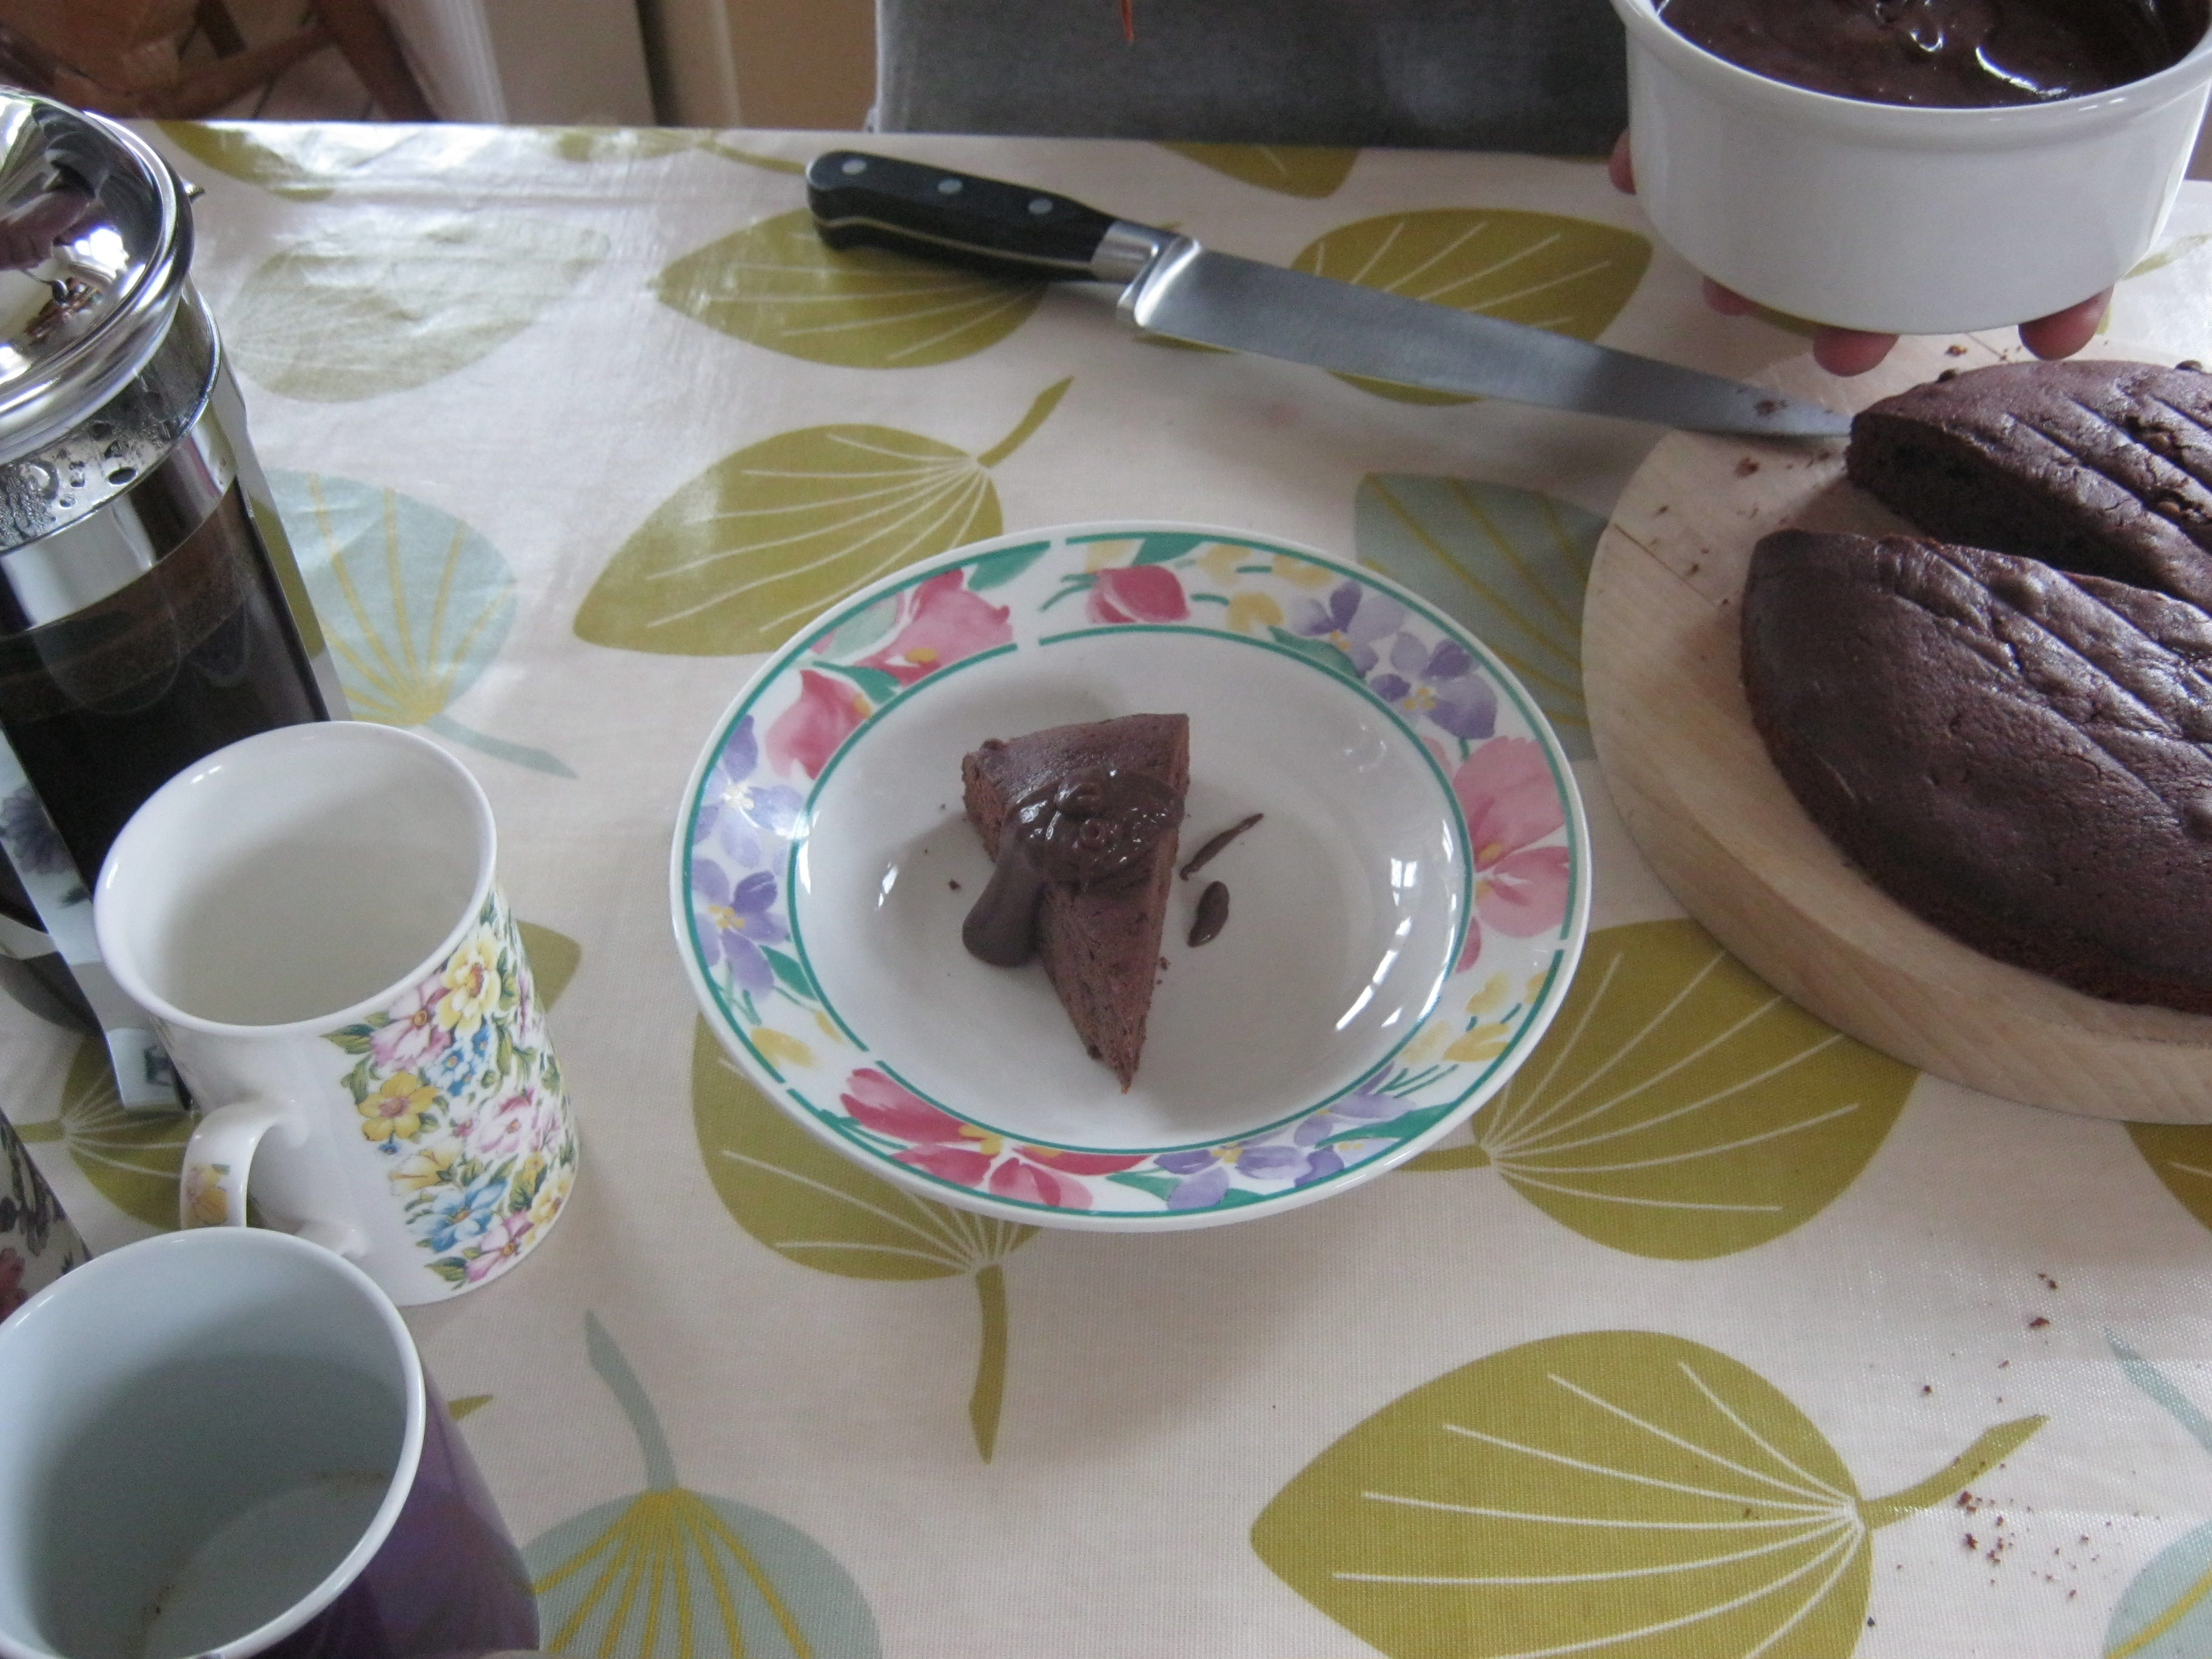
\includegraphics[width=4.5cm]{figures/chef_cake.jpg}
    %         %     \caption{\scriptsize Ciasto ,,HelloWorld'' autorstwa Mike Worth}
    %         % \end{figure}
	% 	\end{column}

	% \end{columns}

\end{frame}
